En este anexo se va a llevar a cabo una explicación mas extensa de algunos de los apartados de la programación que hubieran resultado muy densos o complejos en la explicación del código. Además se hará una descripción más profunda de las tecnologías usadas en la aplicación.

En este anexo solo se utilizarán los extractos de código que acompañen a una explicación o aclaración. Tanto código completo de la aplicación como éste documento están almacenados en un repositorio online de la página de Github para un acceso rápido y cómodo a través del siguiente enlace: \url{https://github.com/IonutMorariu/PV-Calculator}

\section{Descripción de tecnologías}

En desarrollo de cualquier aplicación web intervienen dos partes muy diferencias, cada una con unas funciones específicas. 

Por un lado es necesario desarrollar un servidor, que en la industria se conoce como Backend, encargado de gestionar la base de datos donde se almacenan los datos, y proveer la información necesaria en todo momento a través de peticiones HTTP \footnote{ \textbf{HTTP:} Protocolo de comunicación para transmitir información a través de la web}.

Por otro lado, para que el usuario pueda interactuar con la página, es necesario desarrollar una interfaz para la web, esto se conoce como Frontend o cliente y es lo que se encarga de recoger la información del usuario a través de un formulario que es posteriormente enviado al servidor. Éste realiza los cálculos necesarios, en este caso todo lo relacionado con la radiación solar, y los devuelve al cliente para mostrar los resultados al usuario.

\subsection{Servidor}

En el caso del servidor, existe una gran variedad de lenguajes de programación que se pueden utilizar, cada uno con sus ventajas y desventajas.

Los lenguajes más utilizados para la programación de servidores web son:
\begin{itemize}
\item \textbf{Java:} Es quizás el lenguaje de programación de servidores más extendido y usado en la industria
\item \textbf{Python:} Un lenguaje de programación que destaca por su semejanza con el lenguaje natural. Ha adquirido bastante fama en los últimos años en temas relacionados con el aprendizaje máquina
\item \textbf{PHP:} Uno de los lenguajes más extendidos, en parte por ser el que se ha utilizado para programar Wordpress, el gestor de contenido más utilizado.
\item \textbf{Javascript:} Un lenguaje creado para programar páginas web, pero que gracias a un entorno de ejecución desarrollado por Google, se puede utilizar para crear servidores. La popularidad de de este lenguaje viene de la flexibilidad que ofrece, dado que un solo programador puede realizar las dos tareas, servidor y cliente, si conoce este lenguaje. Comúnmente es confundido con Java, pero son totalmente diferentes.
\end{itemize}

El lenguaje escogido en este caso es Javascript, por experiencias anteriores y por la flexibilidad de utilizar un solo lenguaje en ambos casos. Es un lenguaje de programación interpretado, es decir, no es necesario compilarlo con cada cambio, sino que se ejecuta directamente desde el archivo de código, agilizando el desarrollo a riesgos de cometer más errores en vivo. 

El entorno de Javascript que nos permite crear el servidor es NodeJS. Según la descripción de la página web \cite{node_website}, NodeJS fue ideado como un entorno de ejecución de Javascript orientado a eventos asíncronos, diseñado para crear aplicaciones de red escalables.

Para la base de datos también existen multitud de opciones con diferentes ventajas y desventajas. Algunas de las opciones más utilizadas son:
\begin{itemize}
\item \textbf{MySQL:} La base de datos relacional más extendida, aunque por su edad y arquitectura de diseño, carece de muchas funcionalidades necesarias en el estado actual de la web.
\item \textbf{PostgreSQL}: Una base de datos relacional más moderna, y con mas funcionalidad que MySQL, que está en proceso de sustituir.
\item \textbf{MongoDB:} A diferencia de las SQL, MongoDB es una base de datos no relacional, que guarda la información en documentos individuales en lugar de tablas.
\end{itemize}

La similitud entre la sintaxis de las peticiones y los resultados de MongoDB con la de Javascript ha hecho que sea la opción elegida para este proyecto.

\begin{lstlisting}[style=ES6, caption={Ejemplo de una petición en MongoDB}]
		db.inventory.find( {
     		status: "A",
     		$or: [ { qty: { $lt: 30 } }, { item: /^p/ } ]
		} )
\end{lstlisting}

Se puede observar que tiene muchas similitudes con el lenguaje de programación utilizado, a diferencia de SQL que tiene una sintaxis mas particular:

\begin{lstlisting}[style=ES6, caption={Ejemplo de una petición en SQL}]
		SELECT * FROM inventory WHERE status = "A" AND ( qty < 30 OR item LIKE "p%")
\end{lstlisting}

\subsection{Cliente}

Por el contrario que en el servidor, en el cliente no existen opciones a la hora de programar la interfaz. Solamente se pueden usar 3 lenguajes y cada uno de ellos tiene una función específica.

\subsubsection{HTML}

HTML es el lenguaje que se utiliza para establecer la estructura de la página y dotarla de contenido. Es decir, es lo que se utiliza para definir que campos tendrá el formulario, el titulo de la página y cualquier otro tipo de contenido.

La sintaxis de este lenguaje se conoce como lenguaje de marcado, de ahí sus siglas (Hyper Text Markup Language) que se base en una etiquetas concretas que define sus estructura.
\begin{lstlisting}[style=ES6, caption={Ejemplo de una petición en SQL}]
	<!DOCTYPE html>
	<html>
		<head>
			<title>Page Title</title>
		</head>
		<body>
			<h1>Esto es un titulo</h1>
			<p>This is a párafo.</p>
		</body>
	</html> 
\end{lstlisting}

\subsubsection{CSS}

CSS (Cascading Style Sheet) es el lenguaje que se utiliza en una web para proveer de estilo al contenido definido con HTML. Utiliza un sistema de propiedades y valores que heredan de más general a más especifico. 

Al tratarse de simplemente listas de propiedades que se aplican a las diferentes etiquetan de HTML, es bastante común utilizar códigos ya creados para ahorrar tiempo. Estas listas son también conocidas como librerías de componentes. Las más conocidas son Bootstrap \footnote{\textbf{Bootstrap:} \url{https://getbootstrap.com/} }, Bulma \footnote{\textbf{Bulma:} \url{https://bulma.io/} }  y Zurb Foundation \footnote{\textbf{Zurb Foundation:} \url{https://get.foundation/} }

\begin{lstlisting}[style=ES6, caption={Ejemplo de código CSS \label{code:css_example}}]
	body {
  		background-color: lightblue;
	}

	h1 {
  		color: white;
  		text-align: center;
	}

	p {
  		font-family: verdana;
  		font-size: 20px;
	}
\end{lstlisting}

La forma en la que se escribe dicho código es aplicando ciertas reglas u normas de estilo predefinidas a las diferentes etiquetas de HTML. Así, por ejemplo, según el extracto \ref{code:css_example} todo el documento tendrá de color de fondo el azul, o el titulo de la página será verde y alineado al centro.


\subsubsection{Javascript}
Como ya se ha mencionado anteriormente, Javascript es el lenguaje de programación utilizado tanto para el servidor como para el cliente. 

En el caso del cliente no existen otras opciones dado que Javascript es el único lenguaje que los navegadores web utilizados en la actualidad son capaces de interpretar.

A diferencia de HTML y CSS, Javascript es el encargado de otorgarle la lógica y la funcionalidad a la página web, pues es el que realiza la recogida de datos y su posterior envío al servidor para que se lleven a cabo parte de los cálculos.

En el cliente se realizan los cálculos relacionados con la potencia y la energía entregadas, pues no requiere de acceso a la base de datos y por tanto es posible delegar parte de la carga de trabajo que soporta el servidor.


\section{Explicaciones de código}

\subsection{Emplazamiento del usuario}
Uno de los datos más importantes para poder estimar la energía que finalmente podrá producir el generador es el de la radiación solar en el lugar de instalación.Para ello, es necesario conocer las coordenadas geográficas del emplazamiento. Sin embargo, es poco intuitivo pedirle a un usuario que introduzca sus coordenadas, dado que la mayoría desconocen dichos datos.\\
Por lo tanto, la ruta que se ha tomado es la de pedirle al usuario su dirección, o una dirección cercana a su localización, y utilizar la API de Google Maps \footnote{\textit{API Google Maps}: Enlace interactivo al que se le pueden enviar los datos de una dirección y devuelve las coordenadas de latitud y longitud de un emplazamiento.  } para convertir dicha dirección en las coordenadas de latitud y longitud que se necesitan para poder obtener la radiación en dicho lugar.

Este proceso comienza por recoger los datos de la dirección, municipio y código postal a través del formulario que aparece en la página web.

Estos datos son recogidos en el código a través de un nombre único que han recibido:\\
\begin{lstlisting}[style=ES6, caption={Variables correspondientes a los tres campos}]
const addressInput = document.querySelector('#address');
const cityInput = document.querySelector('#city');
const postalInput = document.querySelector('#postal');
\end{lstlisting}

Una vez que tenemos estos datos recogidos en las variables, podemos pedir a la API de Google Maps las coordenadas de latitud y longitud de dicho emplazamiento encadenando las tres variables y una clave única de identificación,  para obtener un enlace único que se corresponde a dicha localización.
\begin{lstlisting}[style=ES6, label={lst:getCoordinates}, caption={Función encargada de solicitar los datos a la API}]
const getCoordinates = async () => {
	const address = addressInput.value.split(' ').join('+');
	const city = cityInput.value;
	const postal = postalInput.value;
	const requestURL = `${googleEndpoint}address=${address},${city},${postal}
										,spain&key=${googleApiKey}`;
	const response = await fetch(requestURL);
	const data = await response.json();
	const info = {
		formattedAdress: data.results[0].formatted_address,
		lat: data.results[0].geometry.location.lat,
		long: data.results[0].geometry.location.lng
	};

	return info;
};
\end{lstlisting}

La función de \textbf{getCoordinates} (\ref{lst:getCoordinates}) recoge el valor de la dirección y reemplaza los espacios con el signo + (formato requerido por la API) y lo concatena con el valor del campo de la ciudad y el código postal. Al final le añade una clave única que identifica la aplicación a la hora de establecer limites de uso y evitar abuso de la API.\\

Una vez creado este enlace único, el código lanza la petición al servicio y retorna con la información que es recogida y se guarda en dos variables \textbf{lat} y \textbf{long} para ser utilizadas posteriormente, a la hora de obtener los datos de irradiación global.

\subsection{Área, inclinación, orientación y nivel de suciedad de la superficie de instalación}

Además de las información de latitud y longitud del emplazamiento, el cálculo de la instalación también requiere de información relacionada con el área, la inclinación, la orientación y el nivel de suciedad de la superficie donde se va a realizar la instalación, para poder realizar una estimación lo mas exacta posible.

Estos valores son recogidos directamente de los campos de la pagina web, al igual que los campos anteriores, sin necesitar ningún trato especial:
\begin{lstlisting}[style=ES6, caption={Variables correspondientes a los campos indicados}]
const slope = document.querySelector('#slope');
const area = document.querySelector('#area');
const orientation = document.querySelector('#orientation');
const dirtLevel = document.querySelector('#dirt-level');
\end{lstlisting}

\subsection{Obtención de la información de radiación global en el plano horizontal}

En la sección teórica se menciona brevemente como se obtuvo la radiación global en el plano horizontal de manera dinámica en función de la latitud y longitud del emplazamiento.

En ésta sección se va a llevar a cabo un desarrollo más extenso del proceso que se llevó a cabo para poder tener acceso a la información.

El proceso comienza con la búsqueda de una fuente de la radiación global. Investigando las diferentes posibilidades, surge la página de ADRASE, un proyecto fundado por el Gruo de Radiación Solar del CIEMAT. En la página web \footnote{ \textbf{ADRASE}: \url{http://www.adrase.com/el-proyecto.html}} se puede encontrar una descripción detallada acerca del proyecto.

En la página de ADRASE podemos encontrar un mapa interactivo de la península, en la que haciendo clic en cualquier punto, nos aparece un enlace con los datos mensuales de radiación, como se puede observar en la figura \ref{fig:mapa_adrase}.

\begin{figure}[ht]
\includegraphics[scale=0.5]{Mapa_ADRASE}
\centering
\caption{Mapa interactivo de radiación
\label{fig:mapa_adrase}}
\end{figure}

Sin embargo, éste mapa no permite tener un acceso dinámico a la información, sin la interacción de un usuario. Además el servicio de ADRASE no ofrece un punto de acceso a los datos, por tanto, la descarga de datos se tiene que hacer previamente y almacenar los datos en la base de datos del servidor.

Cuando se hace clic en el enlace de datos mensuales de radiación global, aparece una ventana emergente con los datos del emplazamiento, como el de la figura \ref{fig:popup_rad}.

\begin{figure}[ht]
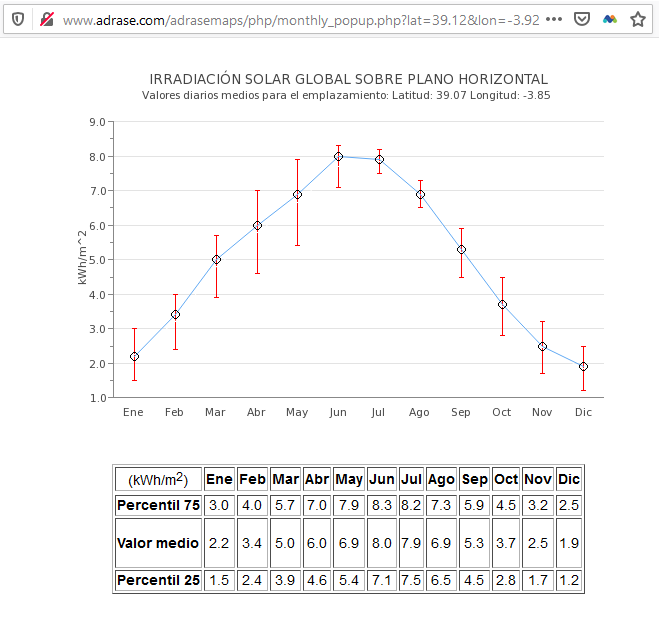
\includegraphics[scale=0.5]{pop_rad}
\centering
\caption{Ventana emergente
\label{fig:pop_rad}}
\end{figure}

La ventana emergente tiene un enlace personalizado de tal manera que pueda generar la información de ese localización concreta. En enlace contiene dos variables que hacen referencia a la latitud y la longitud:

\begin{lstlisting}[style=ES6, caption={Enlace tipo de la radiación en la peninsula}]
www.adrase.com/adrasemaps/php/monthly_popup.php?lat=39.12&lon=-3.92&var_tipe=0
\end{lstlisting}

Por tanto, si generamos un enlace con la latitud y la longitud del emplazamiento, podemos obtener una ventana emergente como la que se muestra en la figura \ref{fig:pop_rad}. Sin embargo, obtener los datos de radiación no es una tarea inmediata. Es necesario procesar el documento y extraer los valores deseados.